% Chapter Template

\chapter{Ensayos y Resultados} % Main chapter title
\label{Chapter4} % Change X to a consecutive number; for referencing this chapter elsewhere, use \ref{ChapterX}

En este capítulo se detallan los resultados esperados y obtenidos sobre etapas puntuales en el trabajo. También se indican las herramientas y metodología
empleadas en cada caso. Finalmente se expone el caso de uso completo integrando todos los componentes que lo componen.



%----------------------------------------------------------------------------------------
%	SECTION 1
%----------------------------------------------------------------------------------------

\section{Pruebas unitarias}

Las pruebas unitarias o \textit{unit testing} son una forma de comprobar que un fragmento de código funciona correctamente. Para este trabajo se programó un \textit{script} utilizando  shUnit2 \citep{WEBSITE:44}, para automatizar diferentes pruebas en la conexión con el broker MQTT.  

Las pruebas unitarias en el backend fueron realizadas teniendo en cuenta las etapas de desarrollo del proyecto y así poder asegurar que en la implementación del frontend no haya problemas en las respuestas a las diferentes consultas.

Por otro lado, se utilizó la herramienta de \textit{testing} que se incluye en Angular para realizar pruebas de la partes más importantes del frontend. 



%----------------------------------------------------------------------------------------
%	Integridad MQTT
%----------------------------------------------------------------------------------------

\subsection{Pruebas de integridad del broker MQTT}

Para hacer pruebas de integridad en el broker MQTT, se instaló shUnit2 y en un \textit{script} se programaron las diferentes pruebas para verificar si la conexión de clientes con el broker MQTT es segura o bien tiene fallas de seguridad. Estas pruebas automatizadas se realizaron mientras se cursaba la materia Ciberseguridad en Internet de las Cosas. 

En el código \ref{cod:script-mqtt} se muestran las diferentes funciones de testeo que se incluyeron en el script. La función de cada una es lograr publicar un mensaje en el broker teniendo en cuenta diferentes etapas de autenticación. 

\begin{lstlisting}[label=cod:script-mqtt,caption=Script para testing de integridad y seguridad de broker MQTT.] 

#! /bin/sh

########################################################################
#	Test para saber si un cliente sin credenciales 
#	puede conectarse - Envio de mensaje prueba_test
########################################################################
testClienteAnonimo(){
 VALUE=$(mosquitto_pub -p 8883 -m prueba_test -t /test -d | grep -o 'PUBLISH') 	
 assertFalse "$VALUE" "PUBLISH"
}

########################################################################
#	Test para saber si un cliente con solo usuario 
#	puede conectarse
########################################################################
testClienteConUsuario(){
 VALUE=$(mosquitto_pub -p 8883 -h localhost -u carlos -m hello -t /test -d | grep -o 'PUBLISH') 
 assertFalse "$VALUE" "PUBLISH"
}


########################################################################
#	Test para saber si un cliente con solo usuario 
#	y password puede conectarse
########################################################################
testClienteConUserYPass(){
 VALUE=$(mosquitto_pub -p 8883 -h localhost -u carlos -P carlos -m hello -t /test -d | grep -o 'PUBLISH') 
 assertFalse "$VALUE" "PUBLISH"
}


########################################################################
#	Test para saber si un cliente puede conectarse
#	con certificados validos
########################################################################
testClienteTLS(){
 VALUE=$(mosquitto_pub -p 8883 --cafile ../ca/ca.crt --cert ../client/client.crt --key ../client/client.key -h localhost -u carlos -P cars -m hello -t /test -d | grep -o 'PUBLISH') 	
 assertEquals "$VALUE" "PUBLISH"
}

\end{lstlisting}

En la tabla \ref{tab:test-mqtt} se describen los tests realizados.

\begin{table}[h]
	\centering
	\caption[Comandos utilizados en MongoDB]{Comandos más utilizados para el manejo de base de datos desarrollada en MongoDB.}
	\begin{tabular}{l p{4.5cm} c }    
		\toprule
		\textbf{Test} 	 										& \textbf{Descripción} 																						& \textbf{Resultado esperado}\\
		\midrule
	
		testClienteAnonimo()			& Verificar si un cliente sin credenciales puede conectarse al broker.    				& Error de conexión\\		
		
		testClienteConUsuario() 			& Verificar si un cliente con nombre de usuario y sin password puede conectarse al broker.    				& Error de conexión\\		
		
		testClienteConUserYPass() 		& Verificar si un cliente con nombre de usuario y password puede conectarse al broker.    				& Error de conexión\\	
		
		testClienteTLS()						& Verificar si un cliente con nombre de usuario y password y certificados puede conectarse al broker.    				& Publicación exitosa\\	
		\bottomrule
		\hline
	\end{tabular}
	\label{tab:test-mqtt}
\end{table}

\pagebreak

Los resultados obtenidos pueden observarse en la figura \ref{fig:mqtt-test}.

\begin{figure}[htpb]
	\centering
	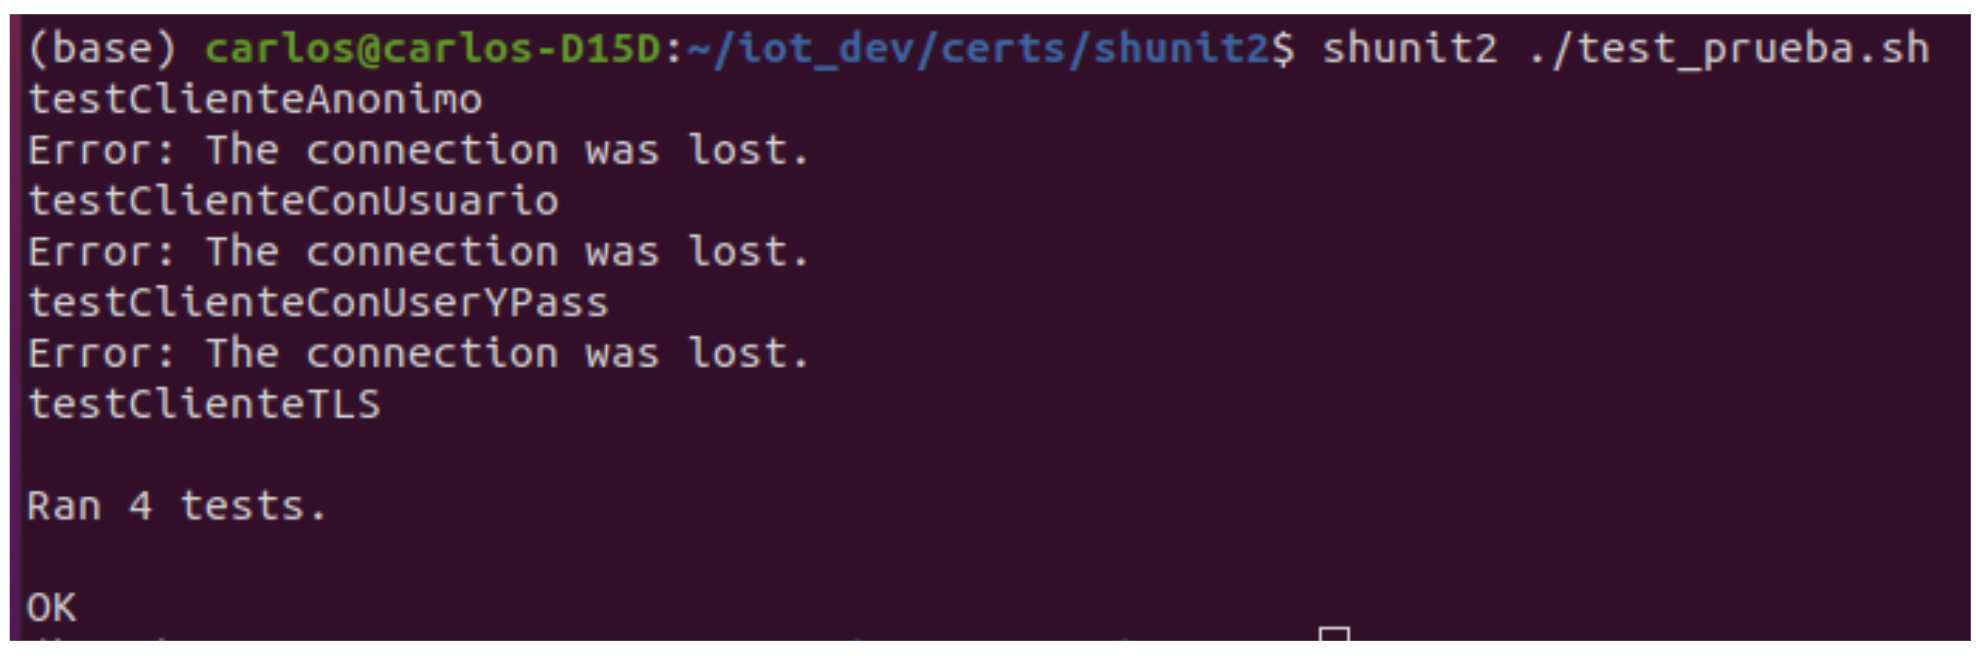
\includegraphics[scale=.35]{./Figures/mqtt-test.png}
	\caption[Testing broker MQTT]{Test de integridad y seguridad del broker MQTT.}
	\label{fig:mqtt-test}
\end{figure}



%----------------------------------------------------------------------------------------
%	Unit Tests
%----------------------------------------------------------------------------------------

\subsection{Pruebas unitarias de funciones del backend}
\label{backend-unit}
Para las pruebas unitarias de las funciones del backend se utilizó el software Postman \citep{WEBSITE:45}, el cual permitió realizar las pruebas de todas las funciones definidas en el backend desde un único sitio. 

En la figura \ref{fig:postman-backend} pueden observarse las carpetas de cada sección de funciones utilizadas en el backend. 

\begin{figure}[htpb]
	\centering
	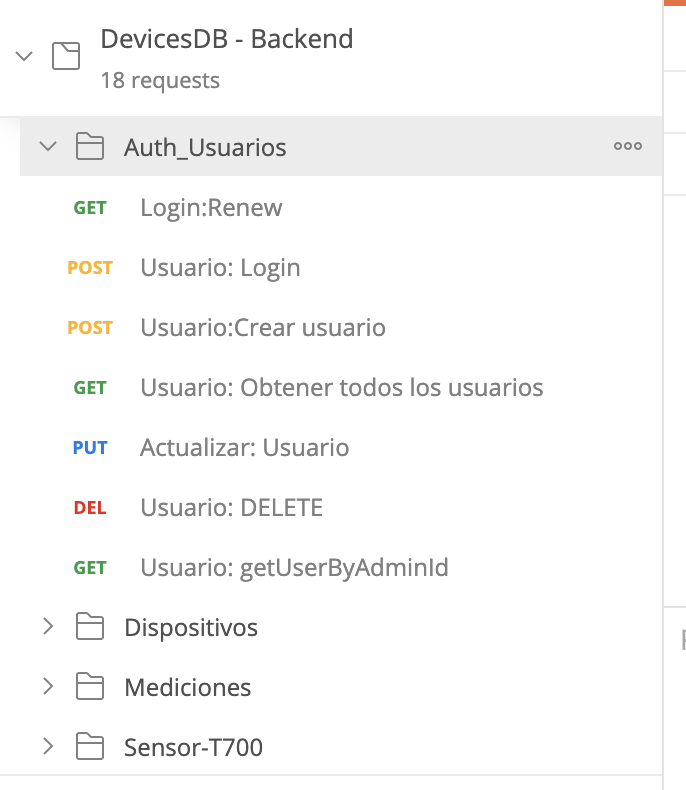
\includegraphics[scale=.56]{./Figures/backend-postman.png}
	\caption[Carpetas de funciones para testing en Postman]{Carpeta con peticiones http para testing de backend en Postman.}
	\label{fig:postman-backend}
\end{figure}

\newpage

Para hacer una petición http al backend, se seleccionó la opción de login de usuario donde se realizó una petición POST pasando como parámetros en el cuerpo del mensaje el email y password como se observa en la figura \ref{fig:postman-login}.

\begin{figure}[htpb]
	\centering
	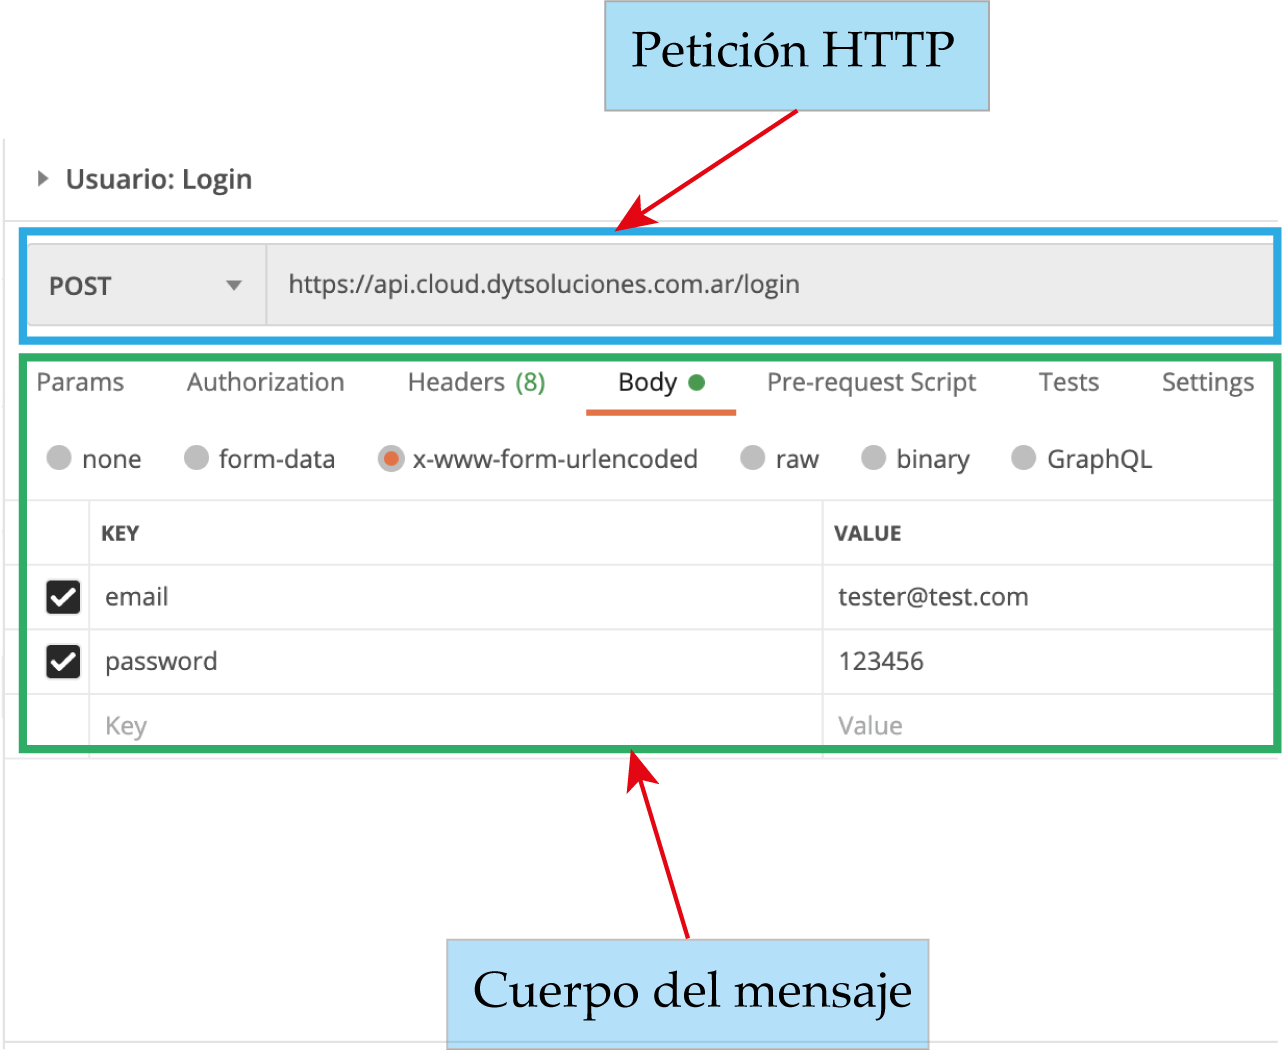
\includegraphics[scale=1.1]{./Figures/postman-login.png}
	\caption[Petición HTTP a función de login de usuarios en Postman]{Ilustración de entorno Postman para hacer una petición POST a la función login de usuario del backend.}
	\label{fig:postman-login}
\end{figure}

\pagebreak
La respuesta a esta petición espera un mensaje en formato JSON con el estado. En caso de ser correcta, se espera un código 200 y además un \textit{token} de acceso para las funciones que lo requieren.  En la figura \ref{fig:login-response} se puede observar la respuesta a la petición POST para el login de usuario.

\begin{figure}[htpb]
	\centering
	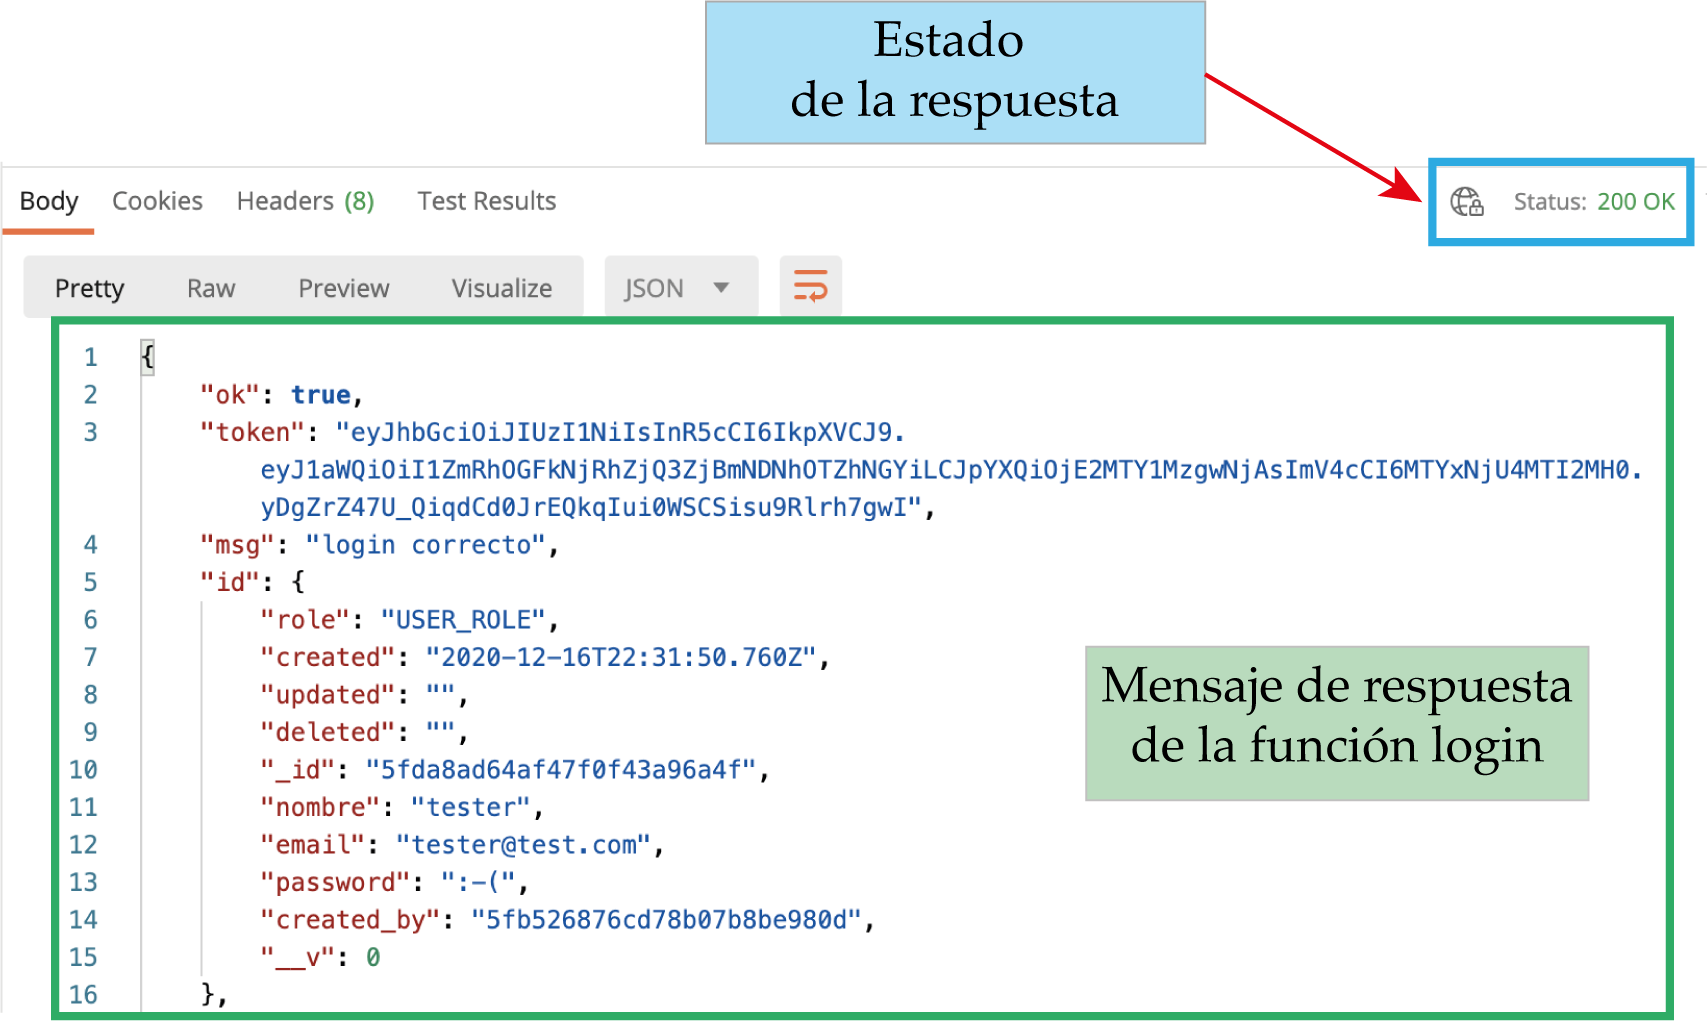
\includegraphics[scale=0.90]{./Figures/login-response.png}
	\caption[Respuesta a petición de login desde Postman]{Ilustración de respuesta del backend a la petición POST de login de usuario en Postman.}
	\label{fig:login-response}
\end{figure}

\pagebreak
Luego del test de login de usuario y de obtener un token, se realizó un test de acceso a funciones del backend que tienen como condición que el usuario envíe un token válido para poder acceder a las respuestas de las mismas. 

El test consistió en realizar la petición con un token inválido esperando un estado de error en su respuesta como se muestra en la figura \ref{fig:not-token-dev}.  

\begin{figure}[htpb]
	\centering
	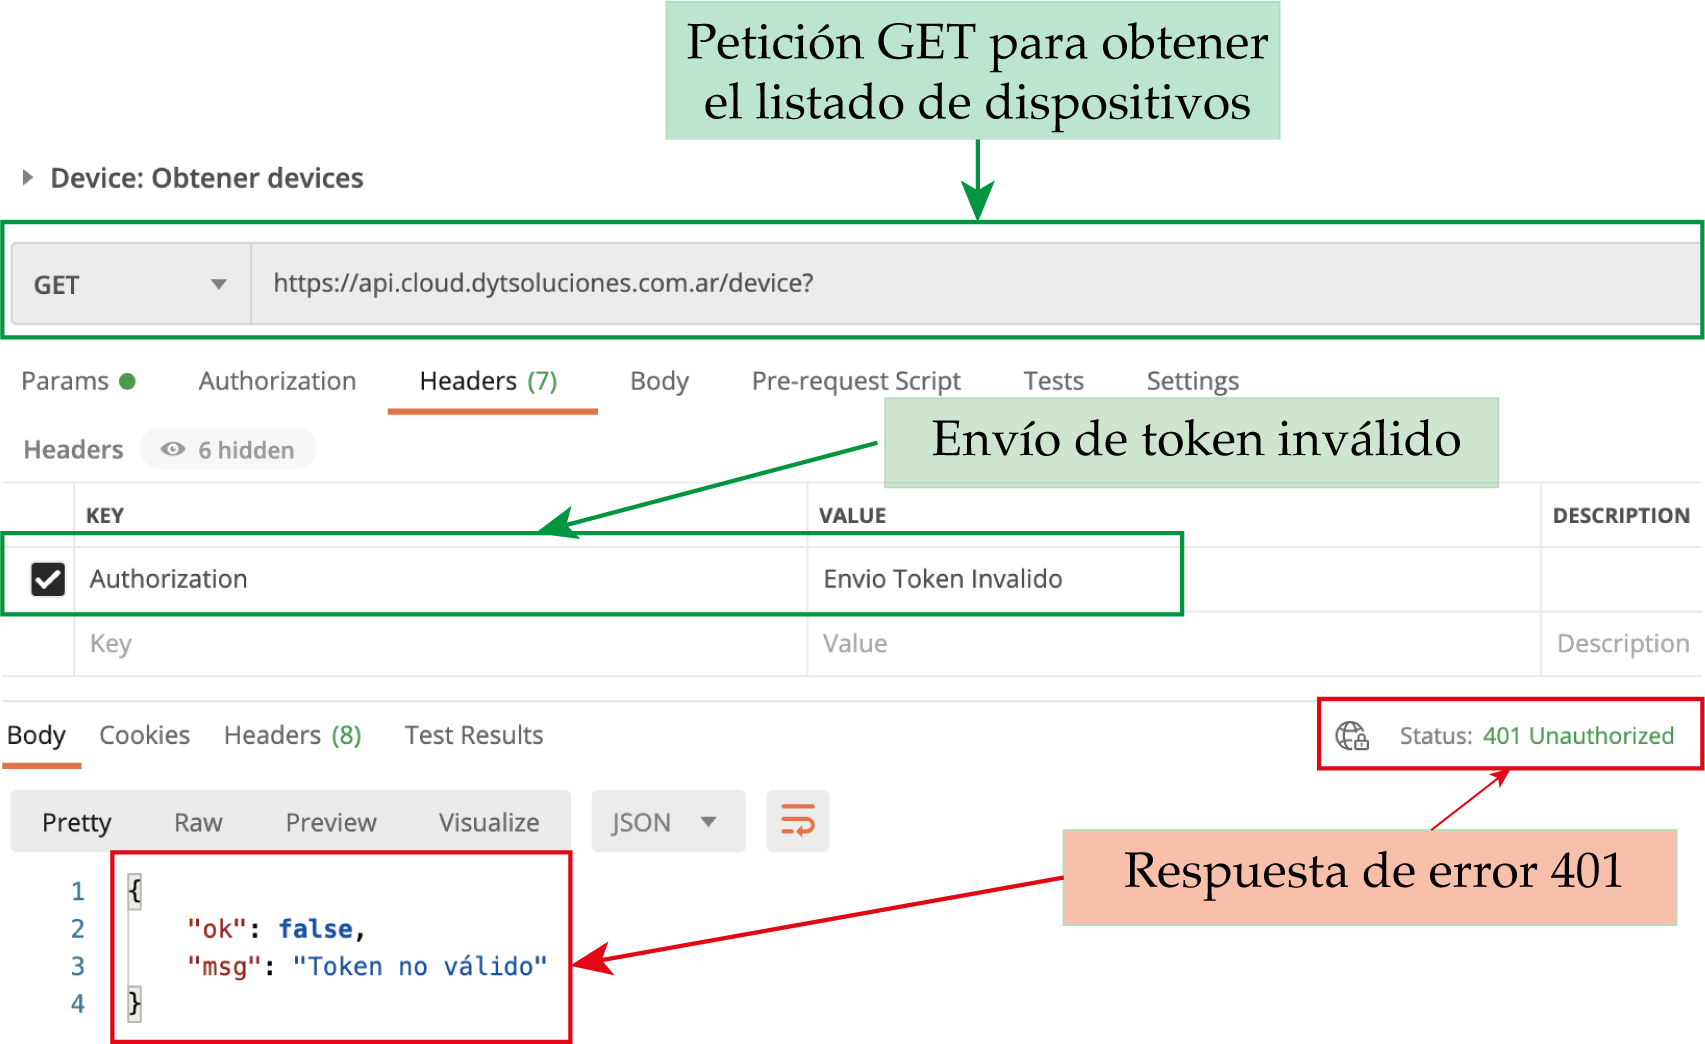
\includegraphics[scale=.90]{./Figures/devices-no-token.png}
	\caption[Respuesta a petición de dispositivos con token inválido]{Ilustración de respuesta del backend a la petición GET de dispositivos con token inválido.}
	\label{fig:not-token-dev}
\end{figure}

\newpage

Por otro lado, en la figura  \ref{fig:valid-token-dev} se realizó la petición de dispositivos al servidor utilizando el token válido adquirido en el login de usuario.



\begin{figure}[htpb]
	\centering
	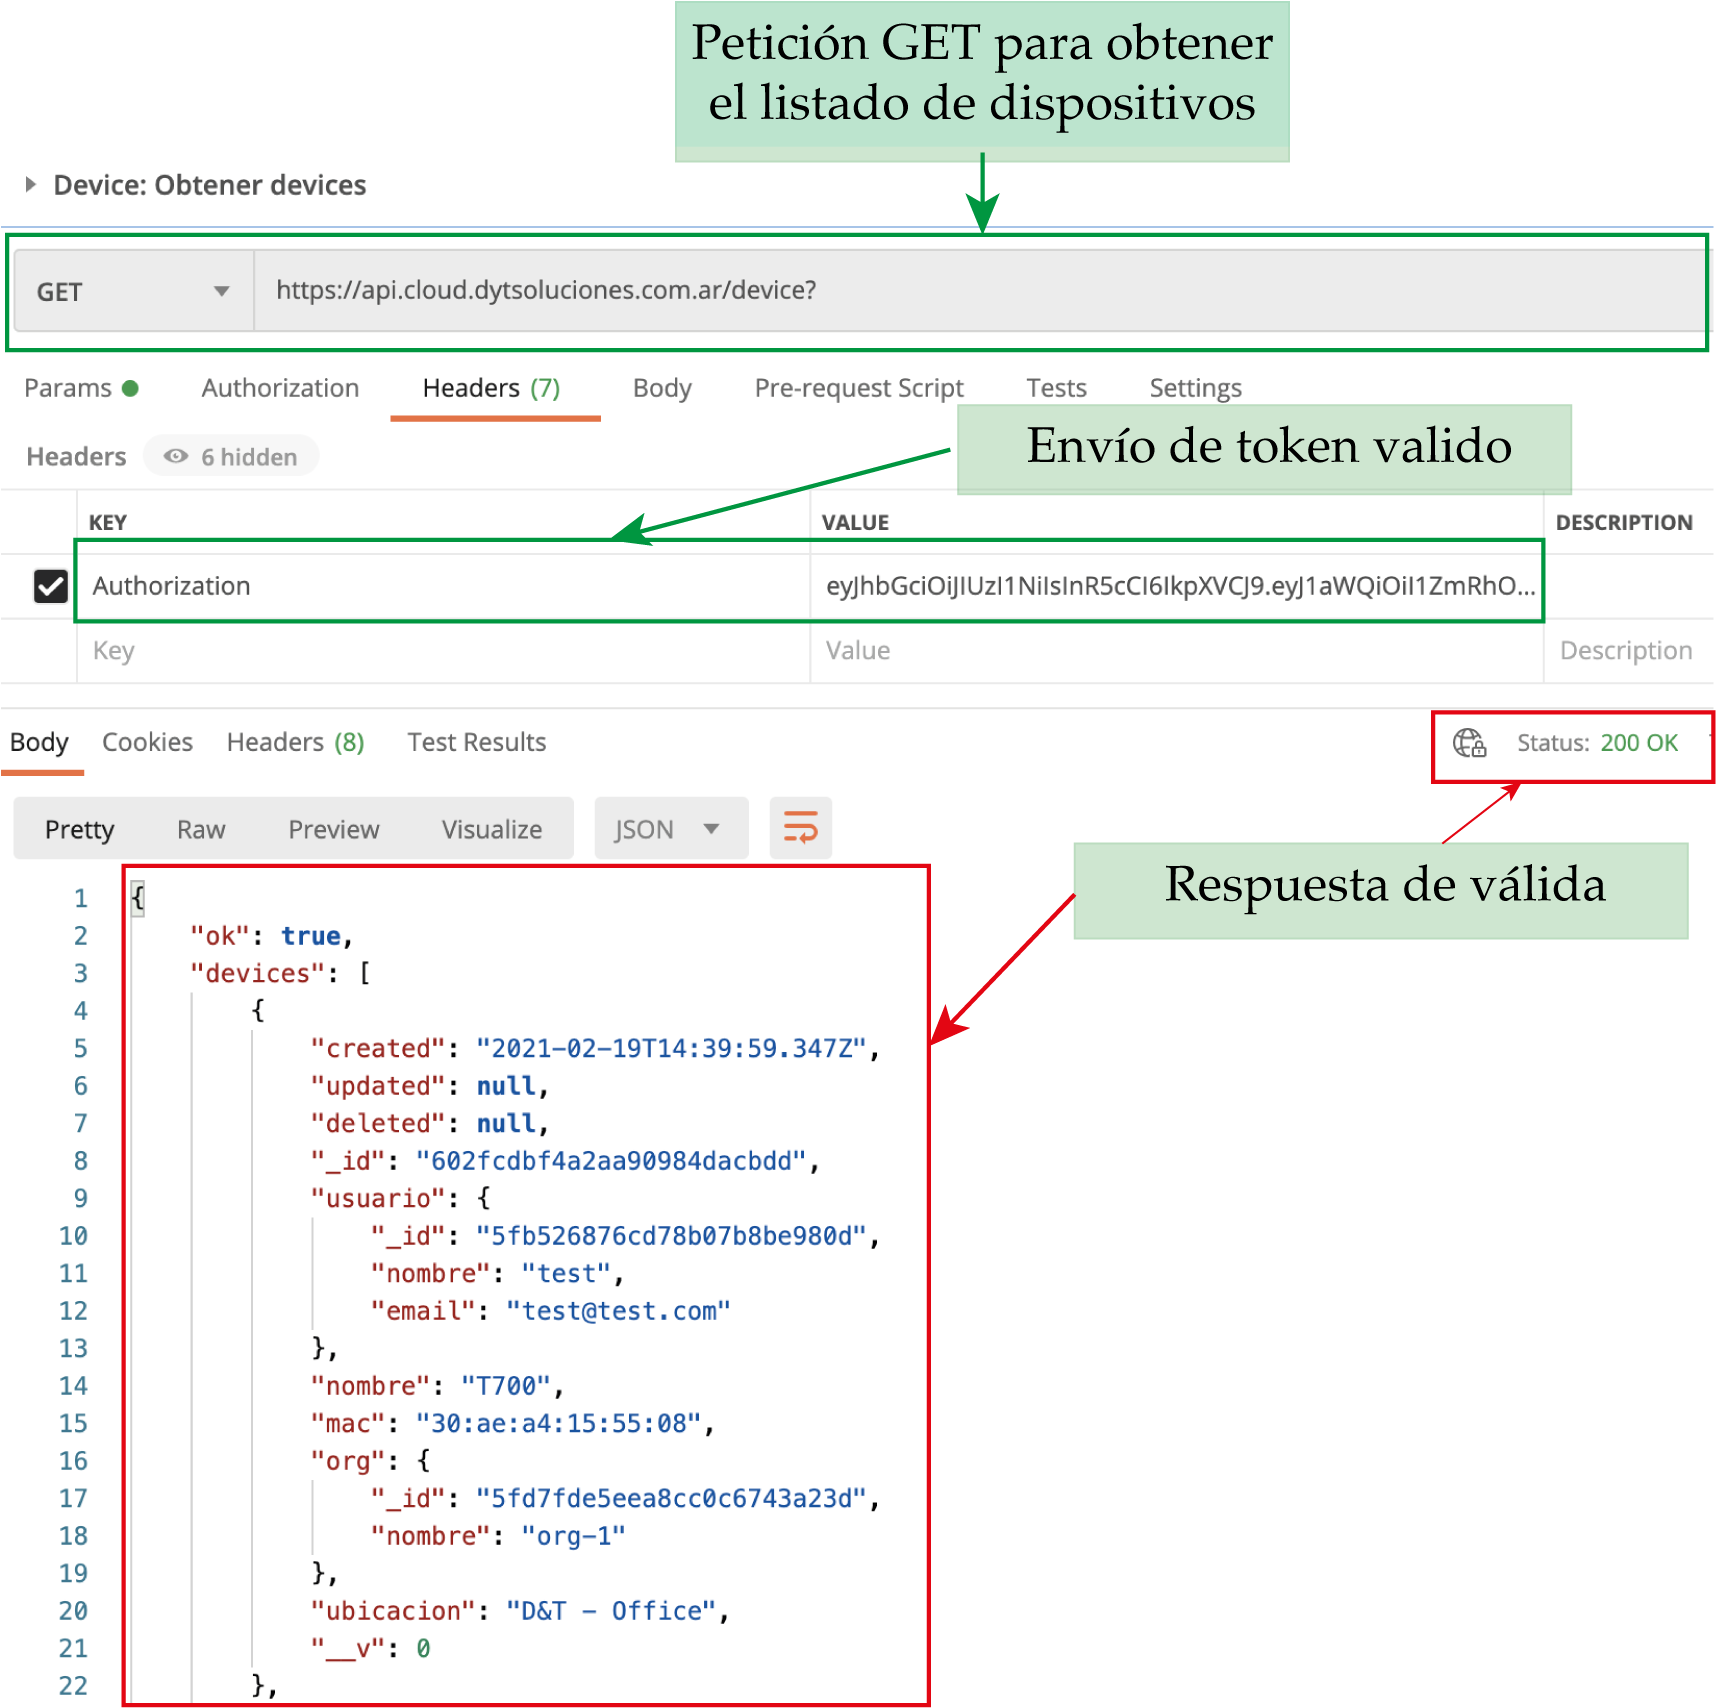
\includegraphics[scale=.90]{./Figures/devices-valid-token.png}
	\caption[Respuesta a petición de dispositivos con token válido]{Ilustración de respuesta del backend a la petición GET de dispositivos con token válido.}
	\label{fig:valid-token-dev}
\end{figure}



%----------------------------------------------------------------------------------------
%	Integration Tests
%----------------------------------------------------------------------------------------

\section{Ensayos de integración}

El objetivo de las pruebas de integración es verificar el correcto funcionamiento entre los distintos componentes del sistema una vez que han sido probados unitariamente.  El fin es comprobar que interactúan correctamente a través de sus interfaces, tanto internas como externas, cubren las funcionalidades establecidas y se ajustan a los requisitos no funcionales especificados en las verificaciones correspondientes.


Para las pruebas de todo el sistema se utilizó la herramienta Cypress \citep{WEBSITE:46} que es un framework que incluye librerías de aserciones, mocks y pruebas e2e \citep{WEBSITE:48} automáticas. Esta herramienta está diseñada especialmente para manejar \textit{frameworks} de Javascript como Angular, Vue, ReactNative, entre otros.

Para la instalación de Cypress sobre Angular, se utilizó npm \citep{WEBSITE:47} y en el código \ref{cod:cmd-cypress} se puede observar el comando utilizado. 

\begin{lstlisting}[label=cod:cmd-cypress,caption=Comando de instalación de Cypress en Angular.] 

npm install cypress --save-dev
\end{lstlisting}

En la figura \ref{fig:cypress-install} se observa la integración de Cypress al archivo de dependencias del desarrollo de Angular  y además la creación de dos archivos para el testeo del sistema en la carpeta de integración. 

\begin{figure}[htpb]
	\centering
	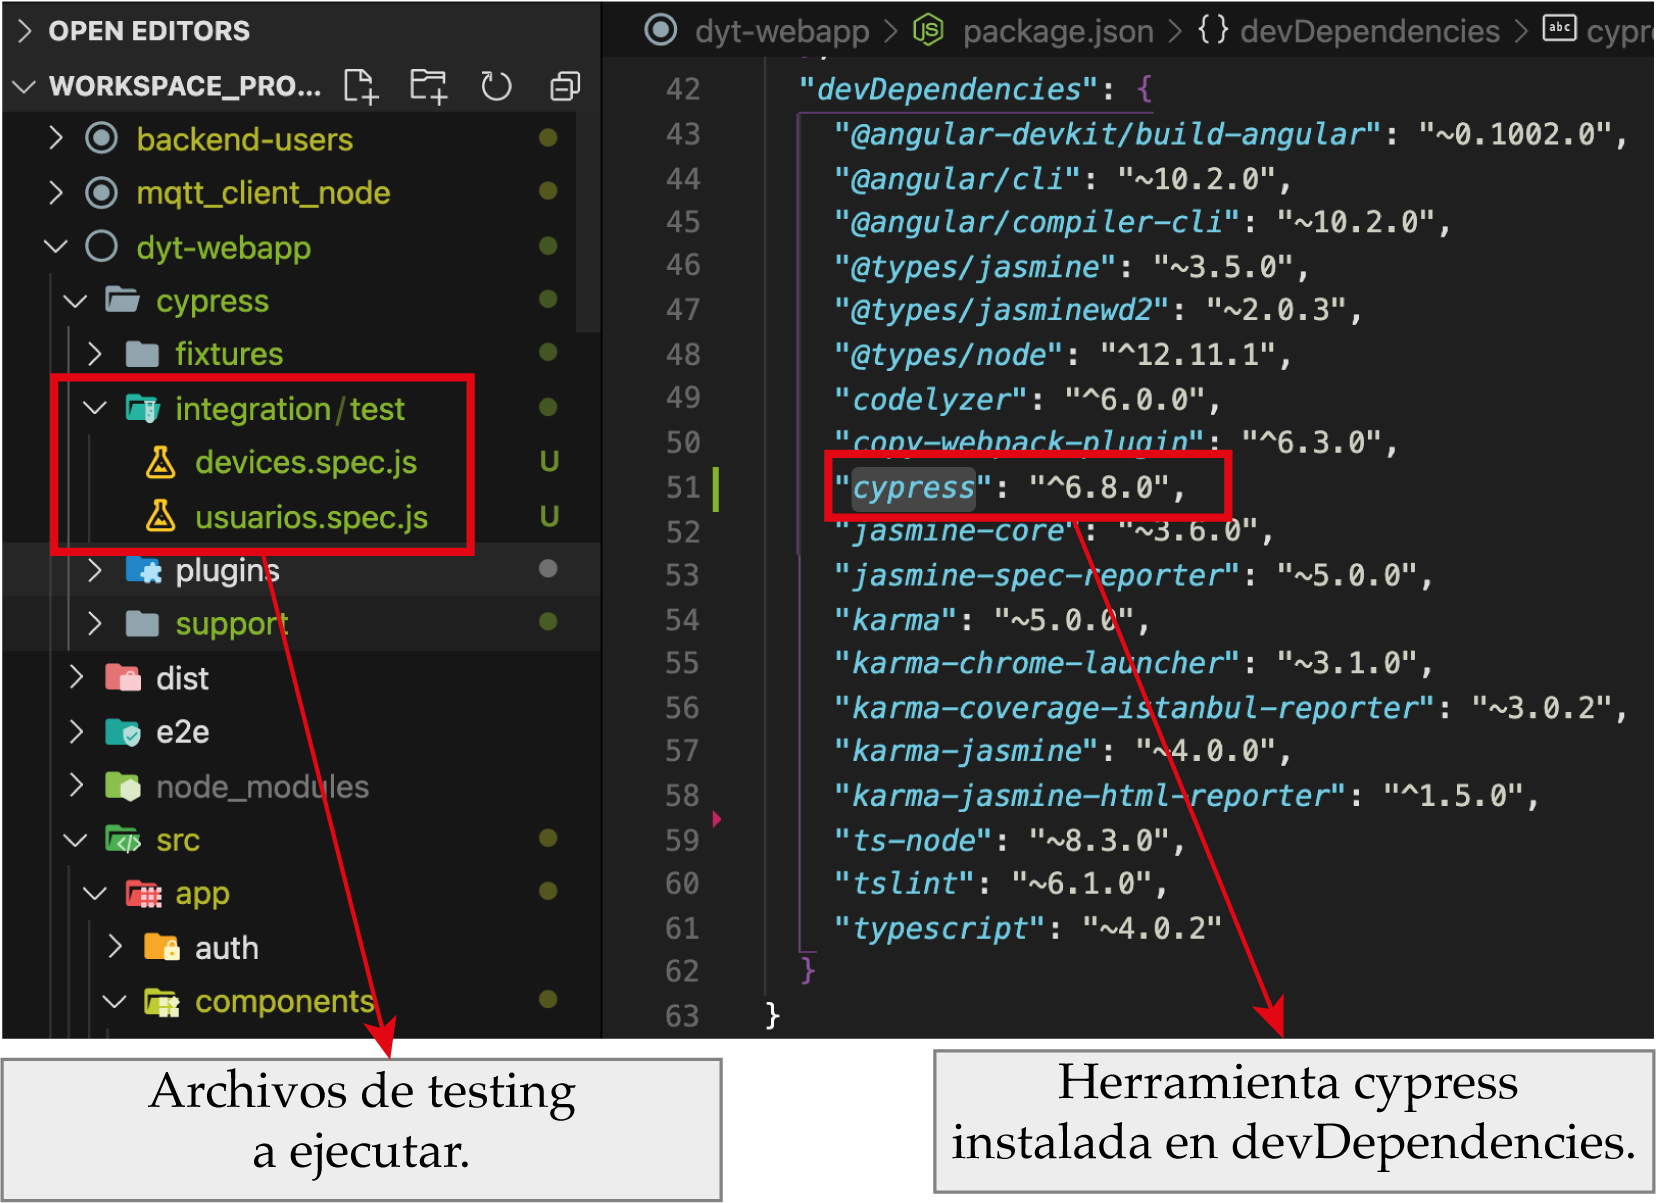
\includegraphics[scale=.9]{./Figures/cypress-install.png}
	\caption[Archivos de instalación de Cypress]{Ilustración archivos de testing generados en carpeta \textit{integration/test} y herramienta instalada en dependencias de desarrollo.}
	\label{fig:cypress-install}
\end{figure}


%----------------------------------------------------------------------------------------
%	Usuarios Integration
%----------------------------------------------------------------------------------------

\subsection{Pruebas de integridad en login de usuarios}
\label{login-tests}
Esta prueba consiste en automatizar los test unitarios que se realizaron en la sección \ref{backend-unit}. Con el uso de Cypress se pudo simular el comportamiento de la pantalla de login de la plataforma web con el usuario, pudiendo observar para cada test, la respuesta que esta pantalla informa al usuario.

En el código \ref{cod:test-login-cypress} se muestra la implementación para los tests que se realizaron en la pantalla de login.

\begin{lstlisting}[label=cod:test-login-cypress,caption=Código de implementación para tests realizados en la pantalla de login de la plataforma web.] 

/// <reference types="cypress" />

context('Test de pagina de login', () => {
  // Antes de cada test, debe visitar la pantalla de login.
  beforeEach(() => {
    cy.visit('http://localhost:4200');
  })


  it('Si el campo email del formulario esta vacio, debe avisar al usuario.', ()=>{
    cy.get('.m-t-40 > .col-xs-12 > .form-control')
      .type('none@test.com').should('have.value', 'none@test.com')
    
    cy.get(':nth-child(3) > .col-xs-12 > .form-control')
      .type('123456').should('have.value', '123456')

    cy.get('#loginform')
      .submit()
      .next()

    cy.get('#swal2-content')
      .contains('Email no encontrado')
  
  });

  it('Si el email ingresado no pertenece a un usuario registrado debe dar un aviso. ', ()=>{
    cy.get('.m-t-40 > .col-xs-12 > .form-control')
      .type('test@test.com').should('have.value', 'test@test.com')
    
    cy.get(':nth-child(3) > .col-xs-12 > .form-control')
      .type('malPass').should('have.value', 'malPass')

    cy.get('#loginform')
      .submit()
      .next()

    cy.get('#swal2-content')
      .contains('Credenciales incorrectas')
  
  });

  it('Si el email ingresado tiene un formato incorrecto, debe avisar al usuario.  ', ()=>{
    cy.get('.m-t-40 > .col-xs-12 > .form-control')
      .type('none!test.com').should('have.value', 'none!test.com')
    
    cy.get(':nth-child(3) > .col-xs-12 > .form-control')
      .type('123456').should('have.value', '123456')

    cy.get('#loginform')
      .submit()
      .next()

      cy.get('.col > p')
        .contains('Debe especificar un email valido')
  
  });

  it('Si el campo del password del formulario esta vacio, debe avisar al usuario.  ', ()=>{
    cy.get('.m-t-40 > .col-xs-12 > .form-control')
      .type('none@test.com').should('have.value', 'none@test.com')
    
    cy.get('#loginform')
      .submit()
      .next()

    cy.get('.col > p')
    .contains('Debe especificar un password')
      
  });

  it('Al ingresar un email y password registrado en el sistema, la pagina debe navegar hacia la ruta /dashboard. ', ()=>{
    cy.get('.m-t-40 > .col-xs-12 > .form-control')
      .type('test@test.com').should('have.value', 'test@test.com')
    
    cy.get(':nth-child(3) > .col-xs-12 > .form-control')
      .type('123456').should('have.value', '123456')

    cy.get('#loginform')
      .submit()
      .next()

    cy.contains('Dashboard')
  
  });

  it('Al realizar el login de un usuario registrado, se debe almacenar el token en el localStorage. ', ()=>{
    cy.get('.m-t-40 > .col-xs-12 > .form-control')
      .type('test@test.com').should('have.value', 'test@test.com')
    
    cy.get(':nth-child(3) > .col-xs-12 > .form-control')
      .type('123456').should('have.value', '123456')

    cy.get('#loginform')
      .submit()
      .next()

    cy.window()
      .its("localStorage")
      .invoke("getItem", "token")
      .should("exist");
  
  });
  
});

\end{lstlisting}


La descripción y resultados de los tests realizados fueron los que se detallan en la tabla \ref{tab:test-cypress-login}.

\begin{table}[h]
	\centering
	\caption[Test de login utilizando Cypress]{Diferentes test automáticos en pantalla login de usuario de la plataforma web utilizando Cypress.}
	\begin{tabular}{p{4cm} p{4cm} p{4cm}}    
		\toprule
		\textbf{Test Cypress }  		& \textbf{Descripción}	& \textbf{Resultado}\\
		\midrule
	
		Si el campo email del formulario está vacío, debe avisar al usuario. 			& Presionar el botón login sin completar el campo email del formulario. 				& Mensaje informando al usuario que debe especificar un email válido. \\	
		
		Si el email ingresado no pertenece a un usuario registrado debe dar un aviso.	 			& Realizar el login con un email no registrado en el sistema. 				& Mensaje de error informando al usuario que el email no fue encontrado.\\	
		
		Si el email ingresado tiene un formato incorrecto, debe avisar al usuario.   & Realizar el login con un texto sin el símbolo \@ en el campo email del formulario.		& Mensaje informando al usuario que debe especificar un email válido.  \\
		
		Si el campo del password del formulario está vacío, debe avisar al usuario. 	 & Presionar el botón login sin completar el campo password del formulario.    & Mensaje informando al usuario que las credenciales son incorrectas.\\	
		
		  
		Al ingresar un email y password registrado en el sistema, la página debe navegar hacia la ruta /dashboard.   & Realizar el login con un email y password previamente registrado en el sistema.  & Visualización de la pantalla dashboard en la plataforma web.\\	
		
		Al realizar el login de un usuario registrado, se debe almacenar el \textit{token} en el localStorage. 		& Realizar el login con un email y password previamente registrado en el sistema y verificar si existe el item \textit{token} en el localStorage. 		& El \textit{token} existe en el localStorage del navegador web.\\	
		
		\bottomrule
		\hline
	\end{tabular}
	\label{tab:test-cypress-login}
\end{table}

\pagebreak

Es importante mencionar que no solamente se están automatizando los tests unitarios sino que además se están verificando los componentes HTML de la plataforma así como los datos alojados en la base de datos. Este tipo de tests también se conocen como e2e (\textit{end-to-end}) y replican el comportamiento de los usuarios con el software en un entorno de aplicación completo. Estas pruebas verifican que los flujos que sigue un usuario trabajen como se espera. En la figura \ref{fig:cypress-test-login} se pueden observar desde la interfaz de Cypress los resultados de los tests realizados.

\begin{figure}[htpb]
	\centering
	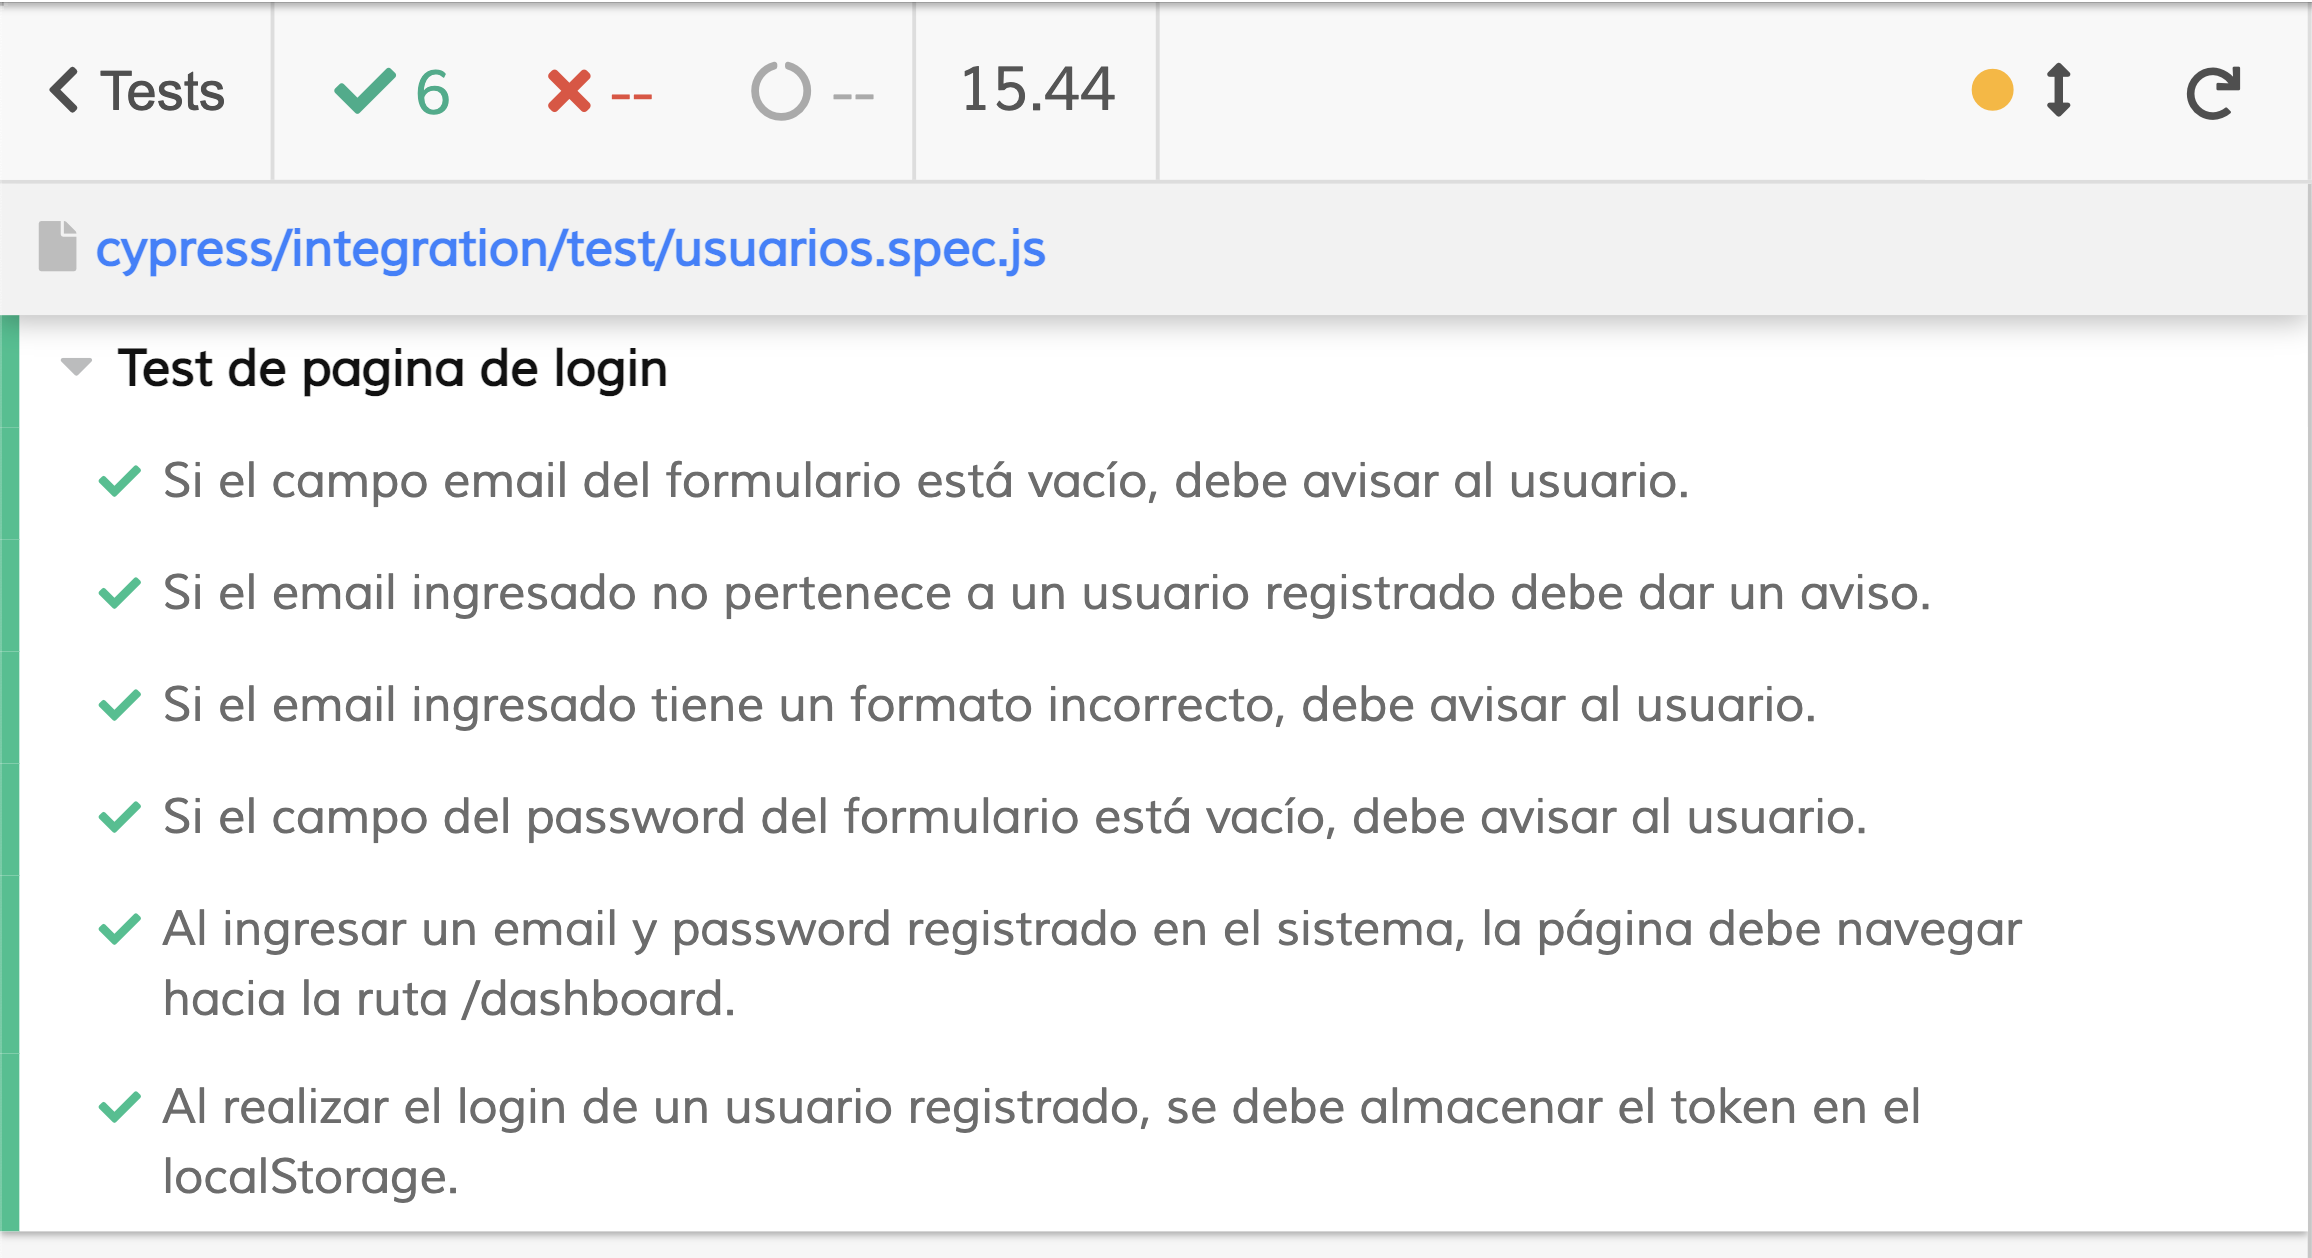
\includegraphics[scale=.30]{./Figures/test-login-cypress.png}
	\caption[Resultado de test de login de la plataforma web]{Ilustración del entorno web de Cypress con los resultados de los test realizados y verificados.}
	\label{fig:cypress-test-login}
\end{figure}

\pagebreak

%----------------------------------------------------------------------------------------
%	Devices Integration
%----------------------------------------------------------------------------------------

\subsection{Pruebas de integridad en dispositivos conectados}
\label{devs-cypress}


Al igual que la sección \ref{login-tests} mediante Cypress se realizaron los tests de integración para los dispositivos del sistema. Una condición a tener en cuenta cuando se realizaron estos tests fue que el usuario llamado test tiene al menos dos dispositivos en su cuenta.  

El código \ref{cod:test-devices-cypress} muestra la implementación de cada una de las pruebas realizadas. 

\begin{lstlisting}[label=cod:test-devices-cypress,caption=Código de implementación para tests realizados en la interacción de usuarios con dispositivos que se encuentran en el sistema.] 

/// <reference types="cypress" />


context('Test de Dispositivos', () => {
    
    Cypress.Commands.add('login', () => { 
        cy.request({
          method: 'POST',
          url: 'https://api.cloud.dytsoluciones.com.ar/login',
          body: {
              email: 'test@test.com',
              password: '123456',      
          }
        })
        .then((resp) => {
        
          window.localStorage.setItem('token', resp.body.token)
          
        })
    })

    // Antes de cada test, debe visitar la pantalla de login.
    beforeEach(() => {
        cy.login()  
    })

    it('En la pantalla del dashboard, deben mostrarse los dispositivos asociados al usuario que realizo el login.', ()=>{
        cy.visit('http://localhost:4200/dashboard');
        cy.contains('Dashboard');

        cy.get(':nth-child(1) > app-t700-sensor > .card > .row > :nth-child(1) > .social-widget > .soc-header')
            .should('exist');
      
    });

    it('Al navegar hacia la pantalla de dispositivos asignados al usuario, debe existir un listado de estos. ', ()=>{
        cy.visit('http://localhost:4200/dashboard/devices');
        cy.contains('Dispositivos')
        cy.get('tbody > tr > td').eq(0)
            .should('contain', 1)
    });

    it('En el dashboard si un dispositivo esta conectado, dl color de su componente no debe ser gris. ', ()=>{
        cy.visit('http://localhost:4200/dashboard');
        cy.contains('Dashboard')       
        cy.wait(10000)
        cy.get(':nth-child(1) > app-t700-sensor > .card > .row > :nth-child(1) > .social-widget > .soc-header', {timeout: 10000})
            .should('have.css', 'background-color', 'rgb(248, 108, 107)')
        
    });

});

\end{lstlisting}


Por otro lado en la tabla \ref{tab:test-cypress-devs} se puede observar la descripción de cada prueba y los resultados obtenidos pueden observarse en la figura \ref{fig:cypress-test-devs}. 
\pagebreak
\begin{table}[h]
	\centering
	\caption[Test de login utilizando Cypress]{Diferentes test automáticos en pantalla login de usuario de la plataforma web utilizando Cypress.}
	\begin{tabular}{p{4cm} p{4cm} p{4cm}}    
		\toprule
		\textbf{Test Cypress }  		& \textbf{Descripción}	& \textbf{Resultado}\\
		\midrule
	
		En la pantalla del \textit{dashboard}, deben mostrarse los dispositivos asociados al usuario que realizó el login.			& Al hacer un login de usuario, la página navega hacia el \textit{dashboart} y se verifica que exista al menos un dispositivo.				& Listado de dispositivos vinculados al usuario que realizó el login.\\	
		
		Al navegar hacia la pantalla de dispositivos asignados al usuario, debe existir un listado de estos. 	 			& Navegar hacia la pantalla /dashboard/devices, verificar que se listen los dispositivos asociados al usuario que realizó el login 				& El primer numero de la lista debe ser igual a uno, indicando que se carga el primer dispositivo.\\	
		
		En el \textit{dashboard} si un dispositivo está conectado, dl color de su componente no debe ser gris.   & Cargar la pagina del \textit{dashboard}, esperar diez segundos para testear si el color del componente del dispositivo cambió a un color diferente del gris indicando que está conectado.		& Se visualiza el cambio de color del componente que identifica a un dispositivo conectado al sistema. \\
		
		
		\bottomrule
		\hline
	\end{tabular}
\label{tab:test-cypress-devs}
\end{table}




\begin{figure}[htpb]
	\centering
	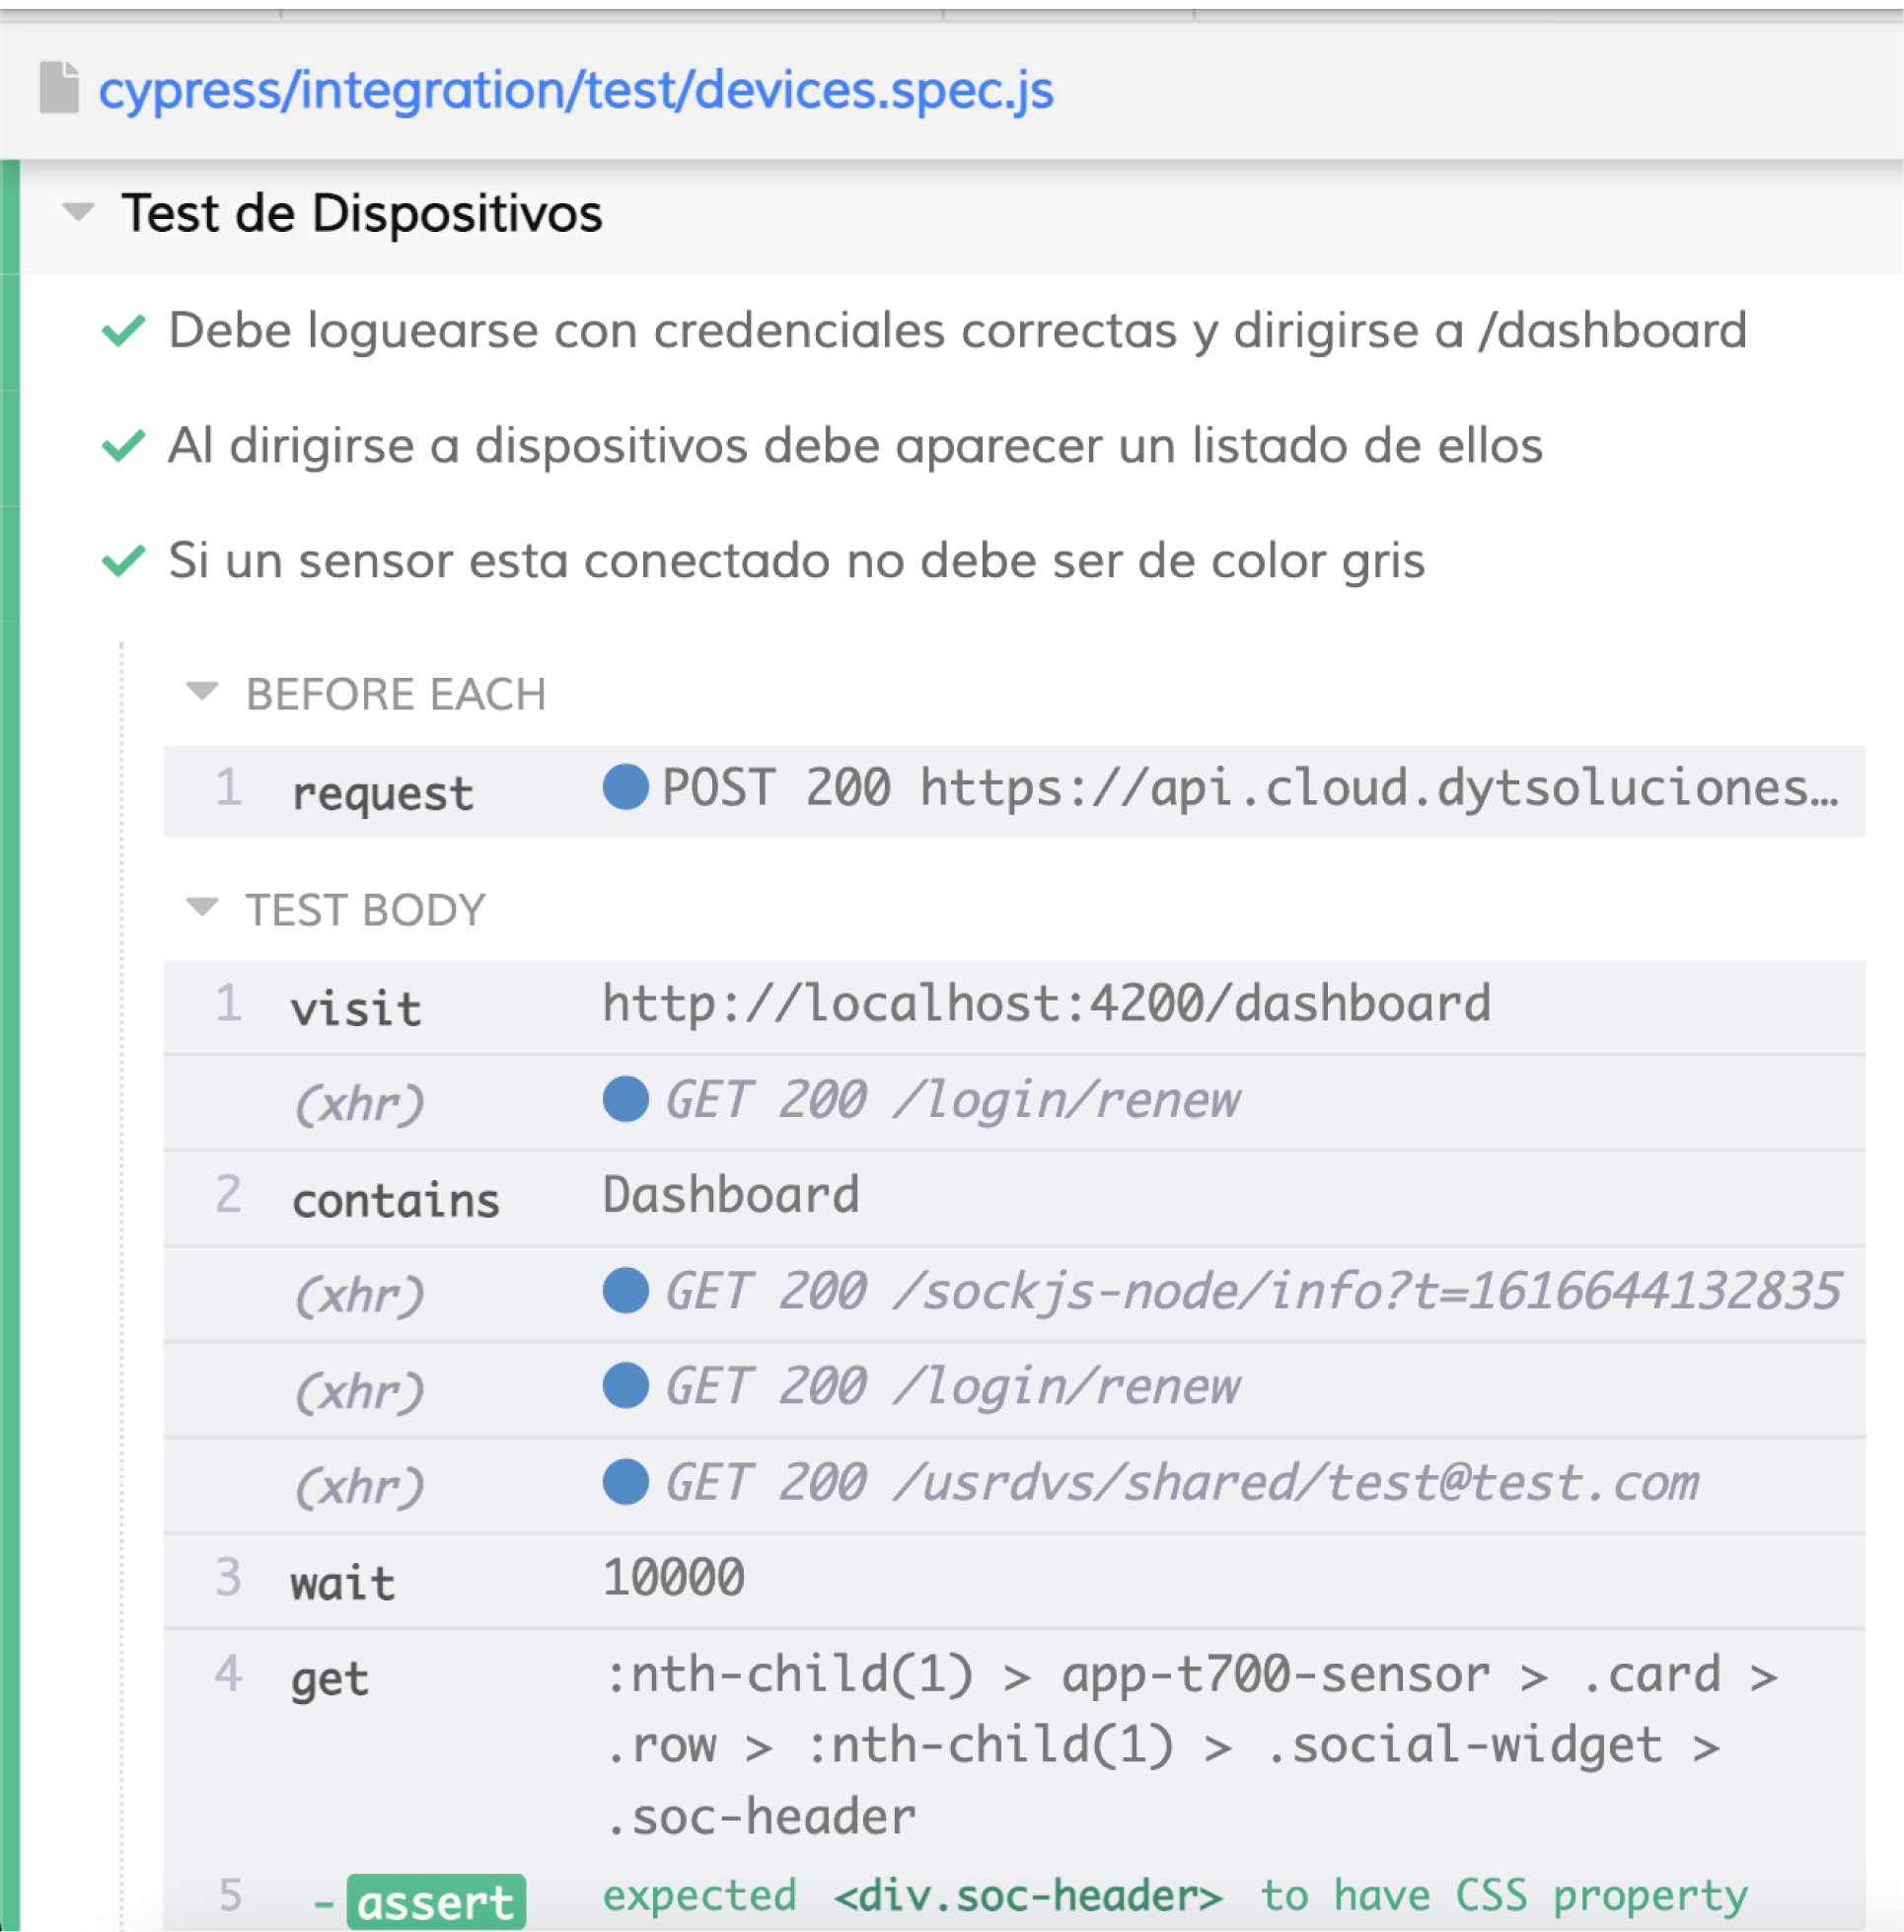
\includegraphics[scale=.60]{./Figures/test-devs-cypress.png}
	\caption[Resultado de test de dispositivos de la plataforma web]{Ilustración del entorno web de Cypress con los resultados de los test realizados a dispositivos asociados a un usuario de la plataforma.}
	\label{fig:cypress-test-devs}
\end{figure}

\pagebreak
Es importante mencionar que se realizó el test de cambio de color del componente de un dispositivo para poder determinar de manera indirecta que el dispositivo está recibiendo datos del broker MQTT.  

En la figura \ref{fig:status-devs} puede observarse los dos estados posibles que pueden tener los dispositivos que se muestran en la pantalla del \textit{dashboard}.  

\begin{figure}[htpb]
	\centering
	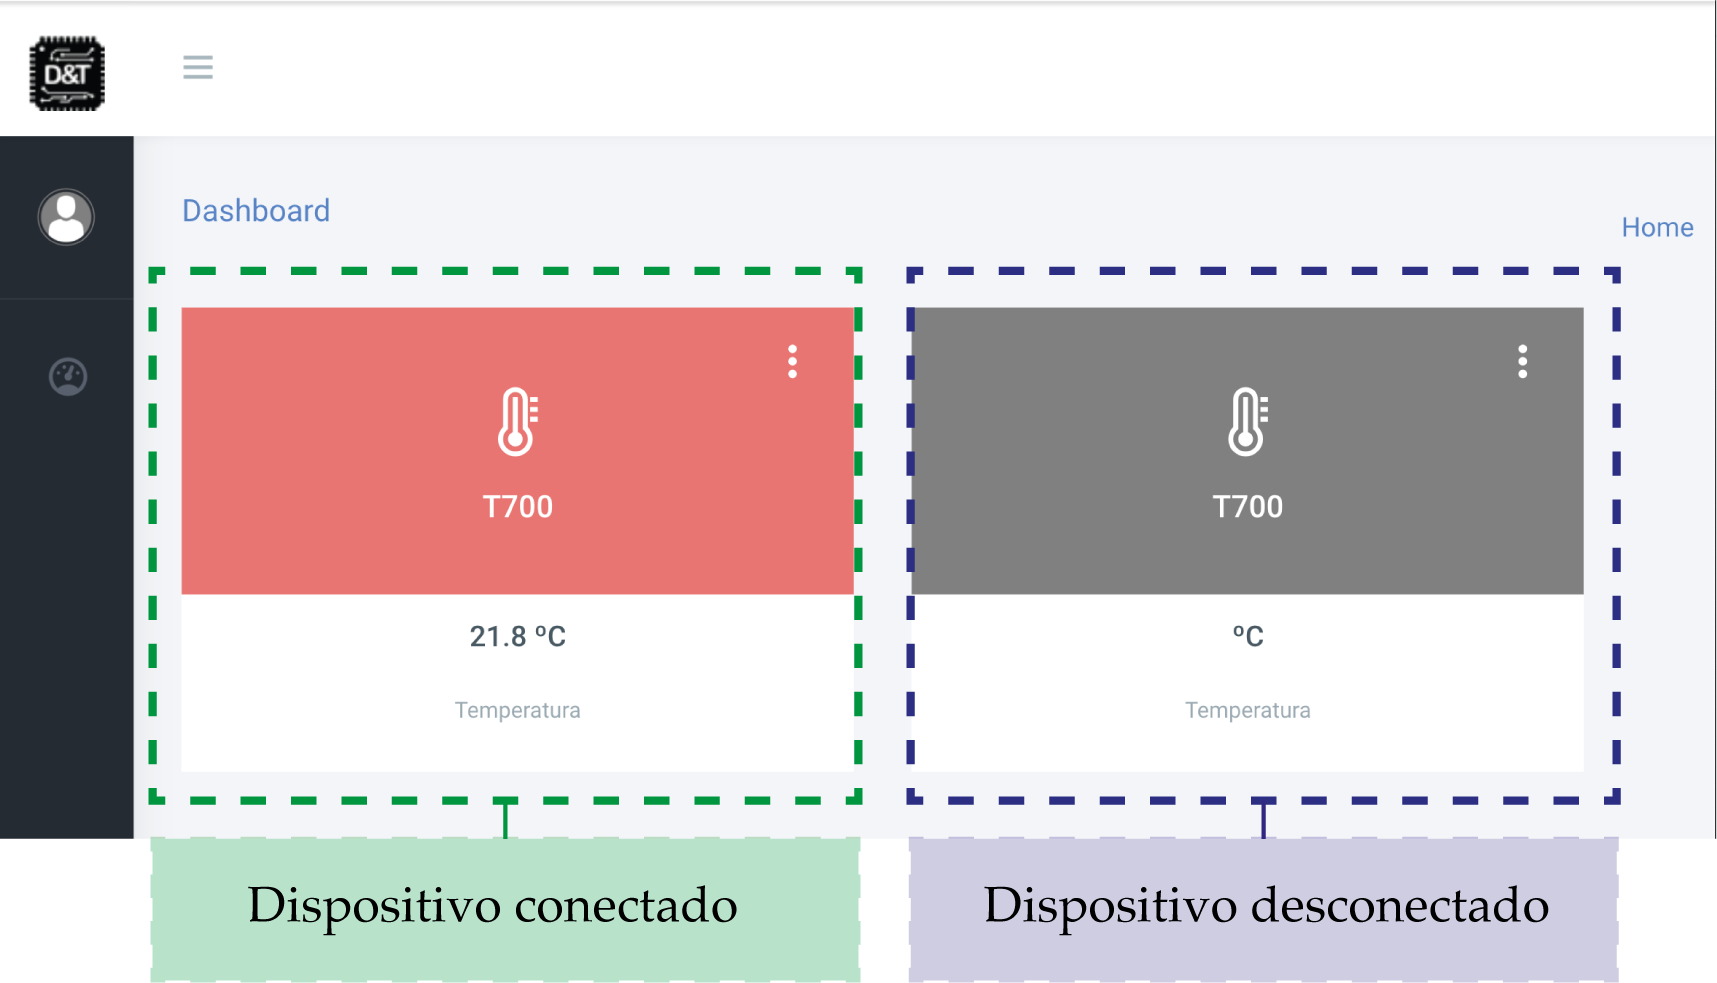
\includegraphics[scale=.75]{./Figures/estado-devs.png}
	\caption[Estados de conexión de componente de dispositivo]{Ilustración los dos estados de conexión que puede obtener el componente que identifica a los dispositivos.}
	\label{fig:status-devs}
\end{figure}

\newpage
%----------------------------------------------------------------------------------------
%	Automatizacion de test
%----------------------------------------------------------------------------------------

\subsection{Ejecución automática de tests realizados }

A fin de automatizar aún más la secuencia de tests de la sección \ref{devs-cypress} y la sección \ref{login-tests}, se agregó en los comandos de ejecución de Angular un comando de Cypress para que realice todas las pruebas que se encuentran contenidas en la carpeta creada para tal fin.  La figura \ref{fig:cmd-e2e} muestra la forma en que Angular ejecutará el comando asignado a la carpeta de test programados. 

\begin{figure}[htpb]
	\centering
	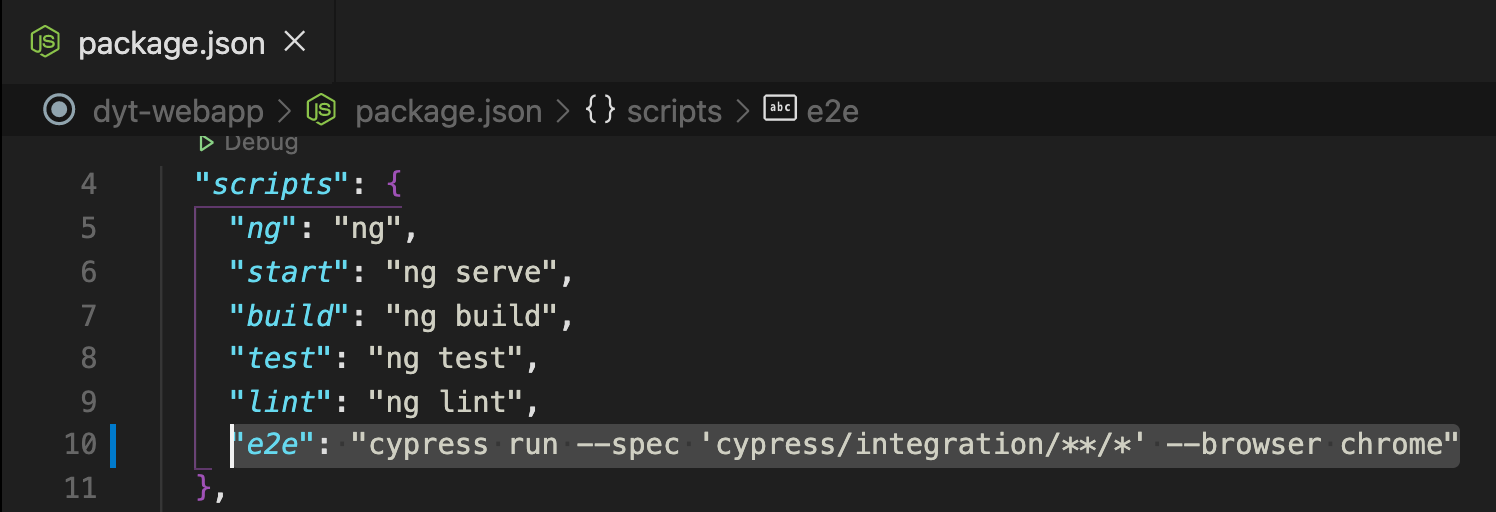
\includegraphics[scale=.50]{./Figures/cmd-e2e.png}
	\caption[Comando en Angular para ejecución de test de Cypress]{Ilustración de comando de ejecución de test e2e de Cypress en el navegador Chrome.}
	\label{fig:cmd-e2e}
\end{figure}


Para ejecutar el test completo, se ingresó el comando que se visualiza en el código \ref{cod:test-all-cypress}.

\begin{lstlisting}[label=cod:test-all-cypress,caption=Comando ejecutado para comienzo de tests programados en cypress.] 
npm run e2e
\end{lstlisting}

\pagebreak
El resultado obtenido se puede observar en la figura \ref{fig:test-all} y se concluye que el resultado de todos los tests fueron los esperados.

\begin{figure}[htpb]
	\centering
	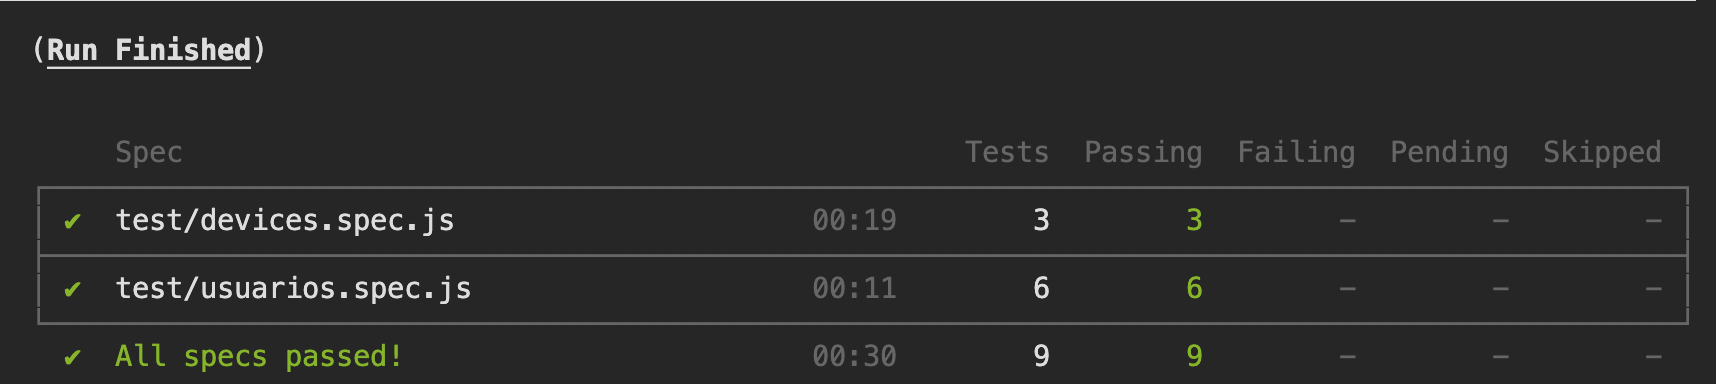
\includegraphics[scale=.45]{./Figures/test-all.png}
	\caption[Resultados de los test ejecutados en Cypress]{Ilustración de respuesta de los test ejecutados en Cypress.}
	\label{fig:test-all}
\end{figure}
